As already mentioned (Section~\ref{sec:introduction}), in the same flavor final state a few additional cuts are added on top of those applied in the opposite flavor.
The proposed new analysis approach is to replace all the SF-specific cuts (except the Z mass veto) with a single cut on the DY MVA output (Table~\ref{tab:ofsfcuts}).

The choice of the working point targets a $\geq$60\% signal increase with respect to 2011 analysis.
Figure~\ref{fig:roc} shows the 2011 analysis working point (WP) as an open square and the DY MVA WP as a full star 
corresponding to a MVA output of 0.6 (0.3) in the 0-jet (1-jet) bin.

It is worth noting that the DY MVA WP has the same signal efficiency as the cut based selection with $p_T$(l2)$>$10 \GeVc\ and \mll$>$12 \GeV;
however, the latter selection has a much larger background efficiency than the DY MVA WP. 
Indeed, comparing the distribution of the selection variables on the signal sample, it is clear that the
main signal recovery comes from \mll\ and $p_T$(l2) with a smaller contribution from min(proj-pfMet,proj-trackMet) (Figures~\ref{fig:gain0j}, \ref{fig:gain1j}).

After the proposed selection, the analysis strategy is mainly unchanged: data/MC scale factors for the main backgrounds are estimated from data
and are used to produce the final yields for the cut based and the shape based analysis; central and alternative shapes are evaluated from data and MC, 
depending on the considered process~\cite{ref:shapenote}. 

The only parts that need to be updated are related to the treatment of the DY background: the DY estimation technique and the evaluation of the DY shape.

%%%%%
\begin{table}[!bh]
\begin{center}
\begin{tabular} {|c|ccc|c|}
\hline
variable & OF cut & SF cut (2011) & SF cut (DY MVA)  & unit \\
\hline
min(proj-pfMet,proj-trackMet)                                 & $>$20 & $>$37+nvtx/2 & $>$20 & \GeV    \\
\mll                                                & $>$12 & $>$20        & $>$12 & \GeVcc  \\
$p_T$(l2)                                           & $>$10 & $>$15        & $>$10 & \GeVc   \\
$p_T$(j1)$<$15 \GeVc\ OR $\Delta\phi$(\Lep\Lep,j1)  & -     & $<$165       & -     & $^\circ$ \\
$|$\mll-$m_Z$$|$                                    & -     & $>$15        & $>$15 & \GeVcc  \\
DY MVA output                                       & -     & -            & WP    &         \\
\hline
\end{tabular}
\caption{Comparison of cuts in 2011 and in the new analysis. WP represents the actual cut value applied on the DY MVA output.}
\label{tab:ofsfcuts}
\end{center}
\end{table}
%%%%%

%%%%%%%%
\begin{figure}[!hbtp]
\begin{center}
\subfigure[0-jet bin]{\label{subfig:roc_0j}
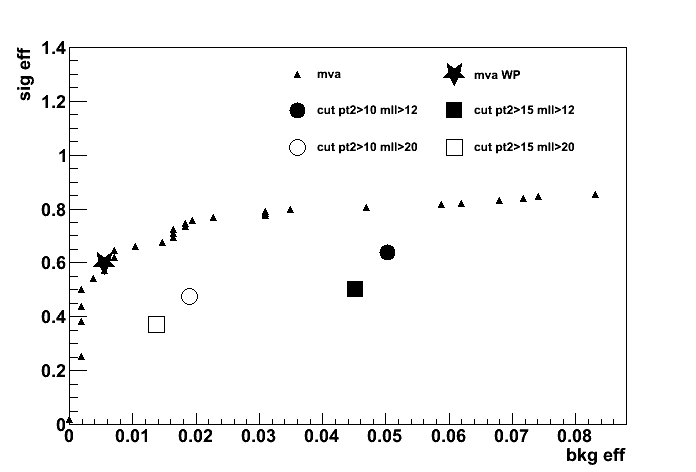
\includegraphics[width=.9\textwidth]{figures/mva_roc0j.png}}\\
\subfigure[1-jet bin]{\label{subfig:roc_1j}
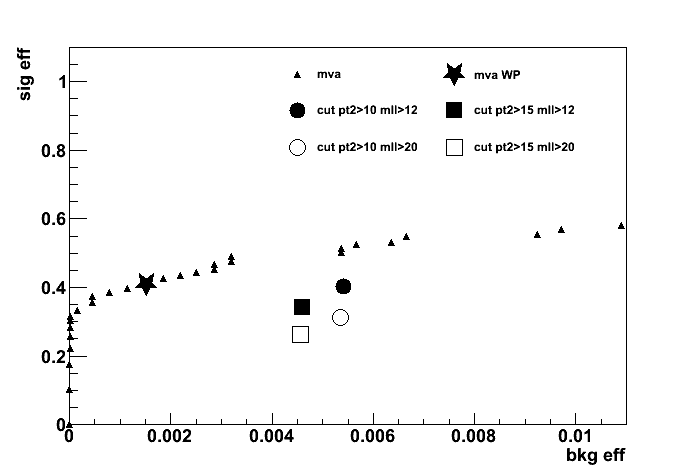
\includegraphics[width=.9\textwidth]{figures/mva_roc1j.png}}
\caption{ROC curve for DY MVA and cut based analysis. The denominator cuts correspond to the training selection plus a cut on \mll$<$70 \GeVcc; 
the numerator includes the numerator plus a cut on DY MVA output for the MVA curve, while for the cut based points 
the cuts on min(proj-pfMet,proj-trackMet) and $\Delta\phi$(\Lep\Lep,j1) from 2011 SF analysis are applied together with the kinematic cuts specified in legenda. }
\label{fig:roc}
\end{center}
\end{figure}
%%%%%%%%

%%%%%%%%
\begin{figure}[!hbtp]
\begin{center}
\subfigure[]{\label{subfig:minmet_0j_hww120}
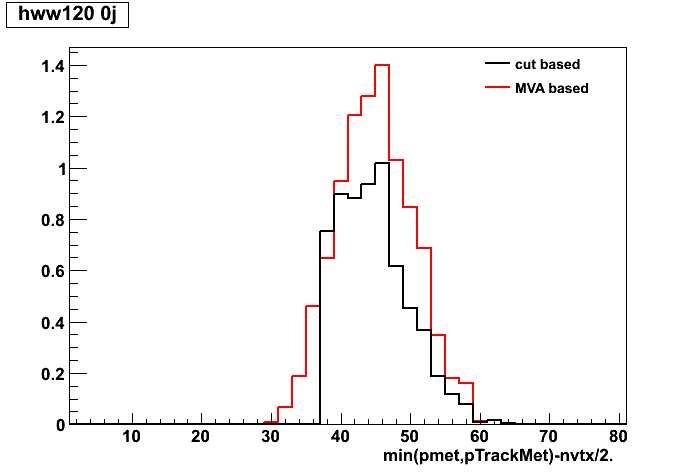
\includegraphics[width=.4\textwidth]{figures/minmet_0j_hww120.png}}
\subfigure[]{\label{subfig:l2pt_0j_hww120}
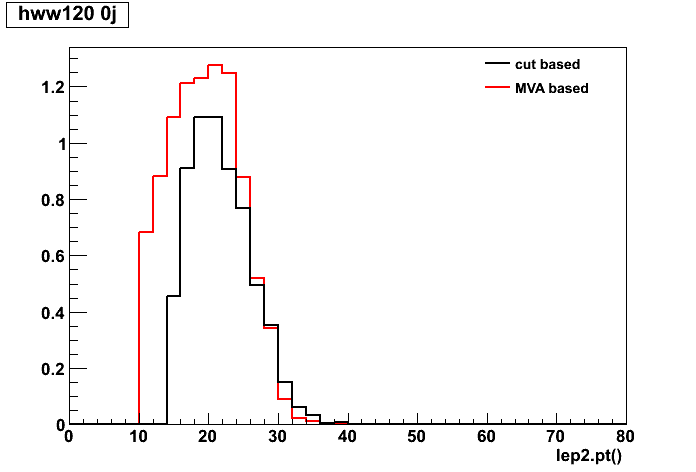
\includegraphics[width=.4\textwidth]{figures/l2pt_0j_hww120.png}}\\
\subfigure[]{\label{subfig:mll_0j_hww120}
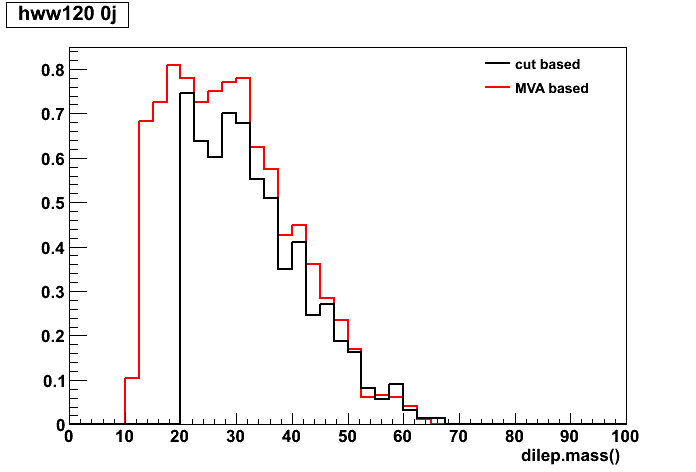
\includegraphics[width=.4\textwidth]{figures/mll_0j_hww120.png}}
\subfigure[]{\label{subfig:dphillj1_0j_hww120}
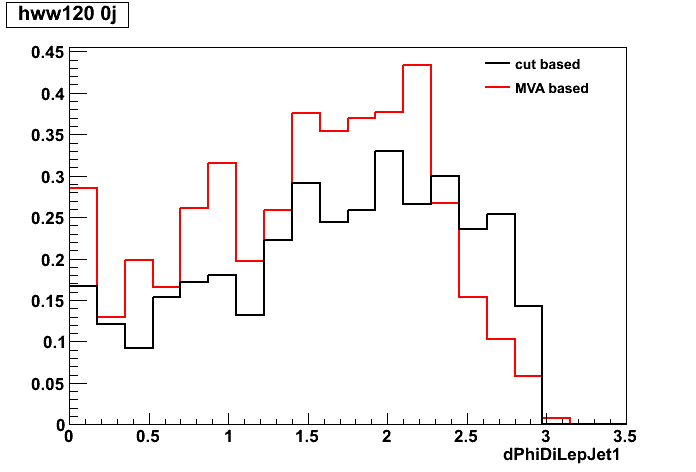
\includegraphics[width=.4\textwidth]{figures/dphillj1_0j_hww120.png}}
\caption{Signal gain with respect to 2011 analysis (0-jet bin).}
\label{fig:gain0j}
\end{center}
\end{figure}
%%%%%%%%

%%%%%%%%
\begin{figure}[!hbtp]
\begin{center}
\subfigure[]{\label{subfig:minmet_1j_hww120}
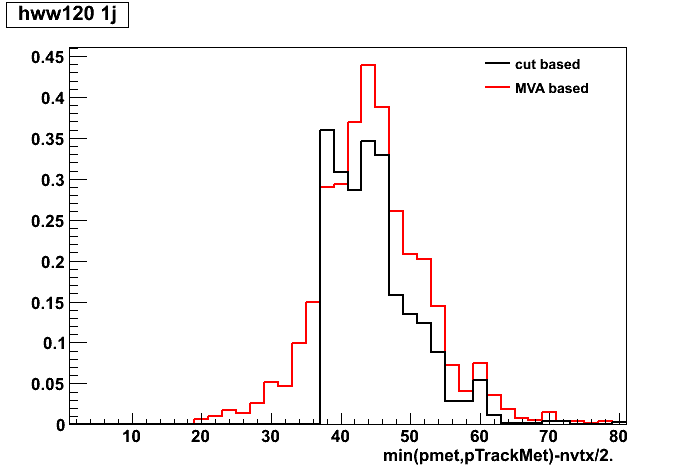
\includegraphics[width=.4\textwidth]{figures/minmet_1j_hww120.png}}
\subfigure[]{\label{subfig:l2pt_1j_hww120}
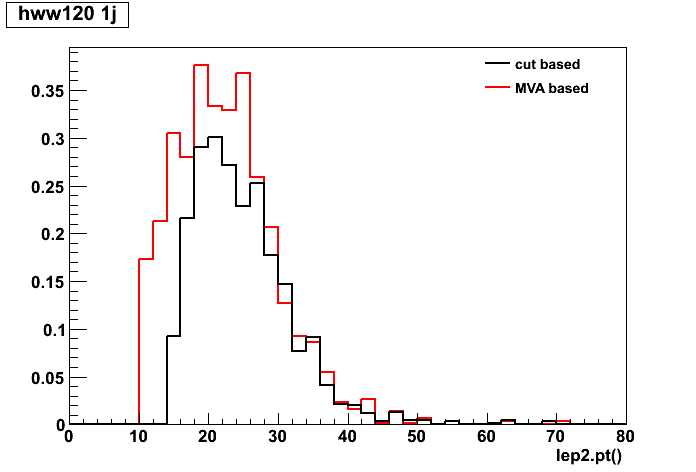
\includegraphics[width=.4\textwidth]{figures/l2pt_1j_hww120.png}}\\
\subfigure[]{\label{subfig:mll_1j_hww120}
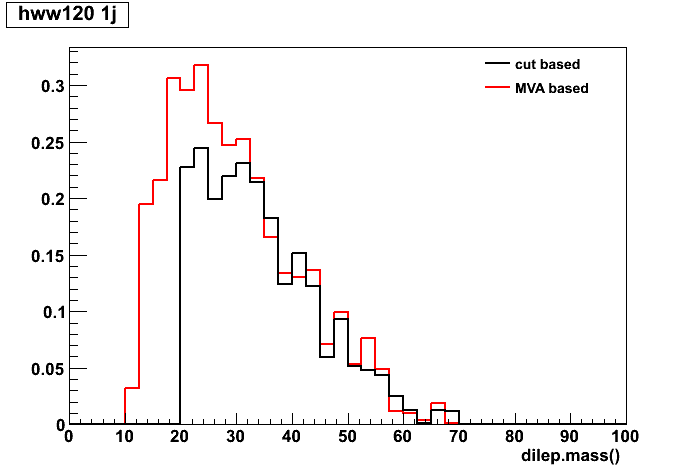
\includegraphics[width=.4\textwidth]{figures/mll_1j_hww120.png}}
\subfigure[]{\label{subfig:dphillj1_1j_hww120}
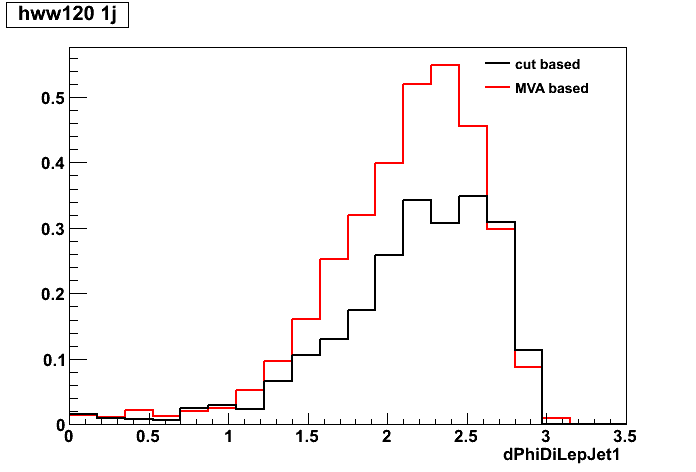
\includegraphics[width=.4\textwidth]{figures/dphillj1_1j_hww120.png}}
\caption{Signal gain with respect to 2111 analysis (1-jet bin).}
\label{fig:gain1j}
\end{center}
\end{figure}
%%%%%%%%

\clearpage

\subsection{DY Background Estimation}

The DY background is evaluated with the \routin\ method: it extrapolates the DY yield under the Z peak to the signal region using a precomputed 
yield ratio (\routin)~\cite{ref:hwwsmurfs}. \routin\ is defined as the ratio of the DY yield in the signal region and the yield under the Z peak. 
In 2011 analysis, it is evaluated on the DY MC sample in four bins corresponding to different \met\ intervals under the assumpion that \routin\ is independent 
from \met\ (Table~\ref{tab:routinbins}).
To reduce the statistical uncertainty, the central value is taken from the 3rd bin and the maximum variation of \routin\ in the \met\ bins is taken as systematic error. 
The limited number of events in the low-mass DY samples led to significant statistical fluctuations in the \routin\ 
determination and, to avoid very large uncertainties, in 2011 analysis a cut on \mll$>$20 \GeVcc\ was applied on SF events. 

The proposed analysis replaces the \met\ cut with a cut on DY MVA output and aims at recovering the signal in the 12$<$\mll$<$20 \GeVcc region.
The definition of \routin\ bins is updated using DY MVA output intervals with equal DY population so that the statistical uncertainty is the same in all bins.
In order to avoid possible problems of MC statistics, we compute \routin\ in data;
both inside and outside the Z peak, the DY contribution is evaluated from the SF yield by subtracting the flavor symmetric backgrounds (\W\W\, Wjets and Top) using OF data 
(corrected for the different selection efficiency of electrons and muons) and subtracting \W\Z\ and \Z\Z\ backgrounds from MC. 
In data, the last bin is possibly contaminated by a Higgs signal and it is not used for the systematic error.
Resulting values of \routin\ are reasonably stable with respect to the considered bin and, despite the limited sample size, they show good data-MC agreement 
(Figure~\ref{fig:routin0j}, ~\ref{fig:routin1j}).

Main consequence of the proposed DY estimation technique is that the cut based analysis does not depend at all on the DY MC. 

%%%%%
\begin{table}[!h]
\begin{center}
\begin{tabular} {|c|c|c|}
\hline
bin & 2011 analysis & DY MVA analysis \\
\hline
1                 & 20$<$\met$<$25 \GeV\ & -0.90$<$DY MVA$<$-0.85 \\
2                 & 25$<$\met$<$30 \GeV\ & -0.85$<$DY MVA$<$-0.60 \\
3                 & 30$<$\met$<$37 \GeV\ & -0.60$<$DY MVA$<$WP    \\
4 (signal region) & \met$>$37 \GeV\      & DY MVA$>$WP            \\
\hline
\end{tabular}
\caption{Definition of bins for \routin\ determination.}
\label{tab:routinbins}
\end{center}
\end{table}
%%%%%

%%%%%%%%
\begin{figure}[!hbtp]
\begin{center}
\subfigure[WW level]{\label{subfig:routin_mh0_0j_newmll12}
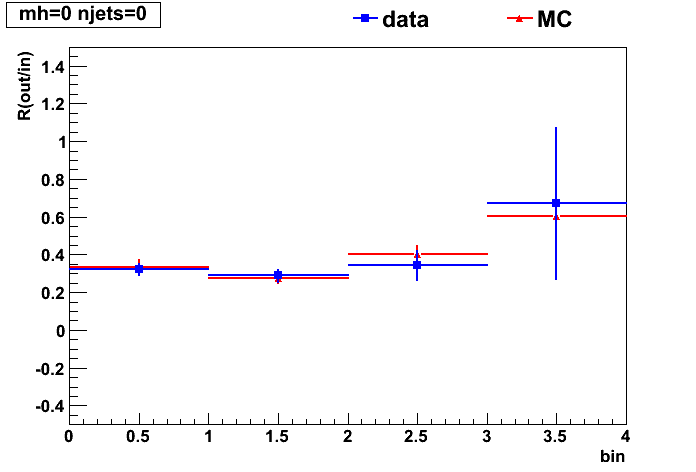
\includegraphics[width=.4\textwidth]{figures/routin_mh0_0j_newmll12.png}}\\
\subfigure[\mHi=120 \GeVcc]{\label{subfig:routin_mh120_0j_newmll12}
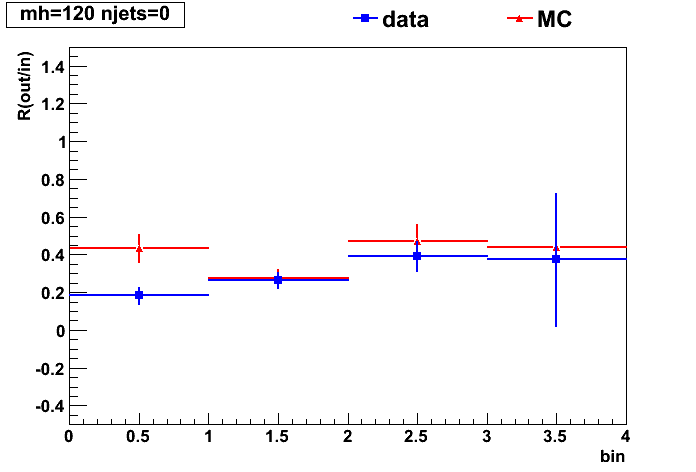
\includegraphics[width=.4\textwidth]{figures/routin_mh120_0j_newmll12.png}}
\subfigure[\mHi=140 \GeVcc]{\label{subfig:routin_mh140_0j_newmll12}
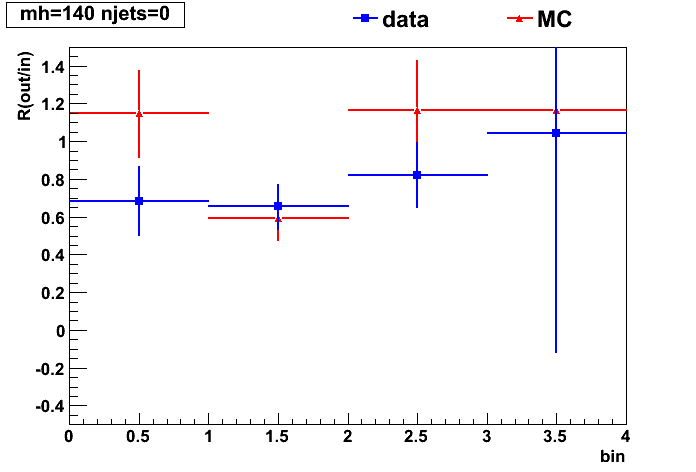
\includegraphics[width=.4\textwidth]{figures/routin_mh140_0j_newmll12.png}}
\caption{\routin\ for DY MVA analysis in the 0-jet bin.}
\label{fig:routin0j}
\end{center}
\end{figure}
%%%%%%%%

%%%%%%%%
\begin{figure}[!hbtp]
\begin{center}
\subfigure[WW level]{\label{subfig:routin_mh0_1j_newmll12}
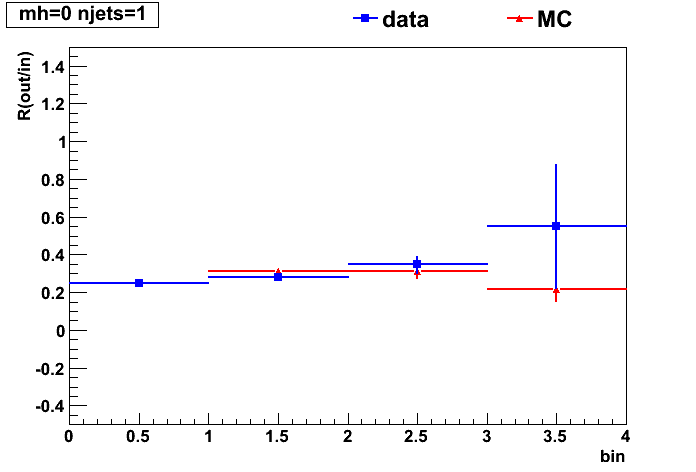
\includegraphics[width=.4\textwidth]{figures/routin_mh0_1j_newmll12.png}}\\
\subfigure[\mHi=120 \GeVcc]{\label{subfig:routin_mh120_1j_newmll12}
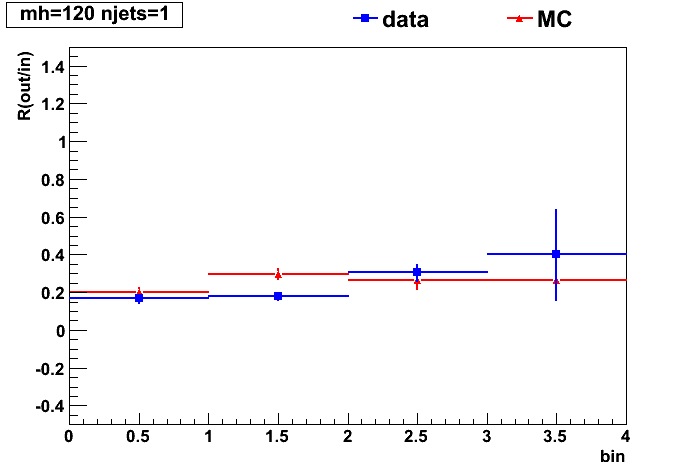
\includegraphics[width=.4\textwidth]{figures/routin_mh120_1j_newmll12.png}}
\subfigure[\mHi=140 \GeVcc]{\label{subfig:routin_mh140_1j_newmll12}
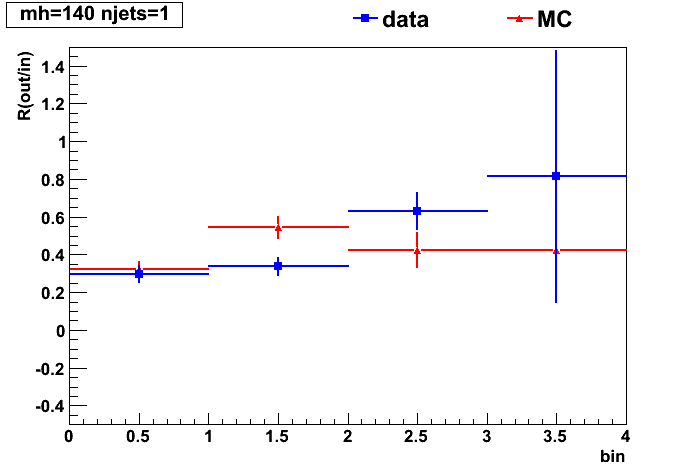
\includegraphics[width=.4\textwidth]{figures/routin_mh140_1j_newmll12.png}}
\caption{\routin\ for DY MVA analysis in the 1-jet bin.}
\label{fig:routin1j}
\end{center}
\end{figure}
%%%%%%%%

\subsection{DY Shape}

The variable used for the shape analysis is the output of another MVA discriminator, trained aginast WW (WW MVA). 
The different WW MVA shape for DY and Higgs events brings additional rejection power in the SF analysis: 
therefore, it is important to check that the cut on DY MVA does not affect the WW MVA shape and the DY and signal shapes are still distinguishable. 
We verified that the WW and DY MVA outputs have linear correlation factors less than 10\% (Figures~\ref{fig:wwmvacorr0j}, \ref{fig:wwmvacorr1j}): this weak correlation
assures that the additional rejection power of WW MVA shape is preserved.

The 2011 shape analysis derive both the central and the alternative shape from MC: the central from the low MET region corresponding to the 3rd bin for \routin\ 
and the alternative the signal region. 
In the present study, we evaluate the central shape from the 3rd bin in data, while we still use MC for the alternative shape: 
this is the only place where the DY MC is directly used in the limit setting procedure.

%%%%%%%%
\begin{figure}[!hbtp]
\begin{center}
\subfigure[Signal]{\label{subfig:0j_mll12_hww120}
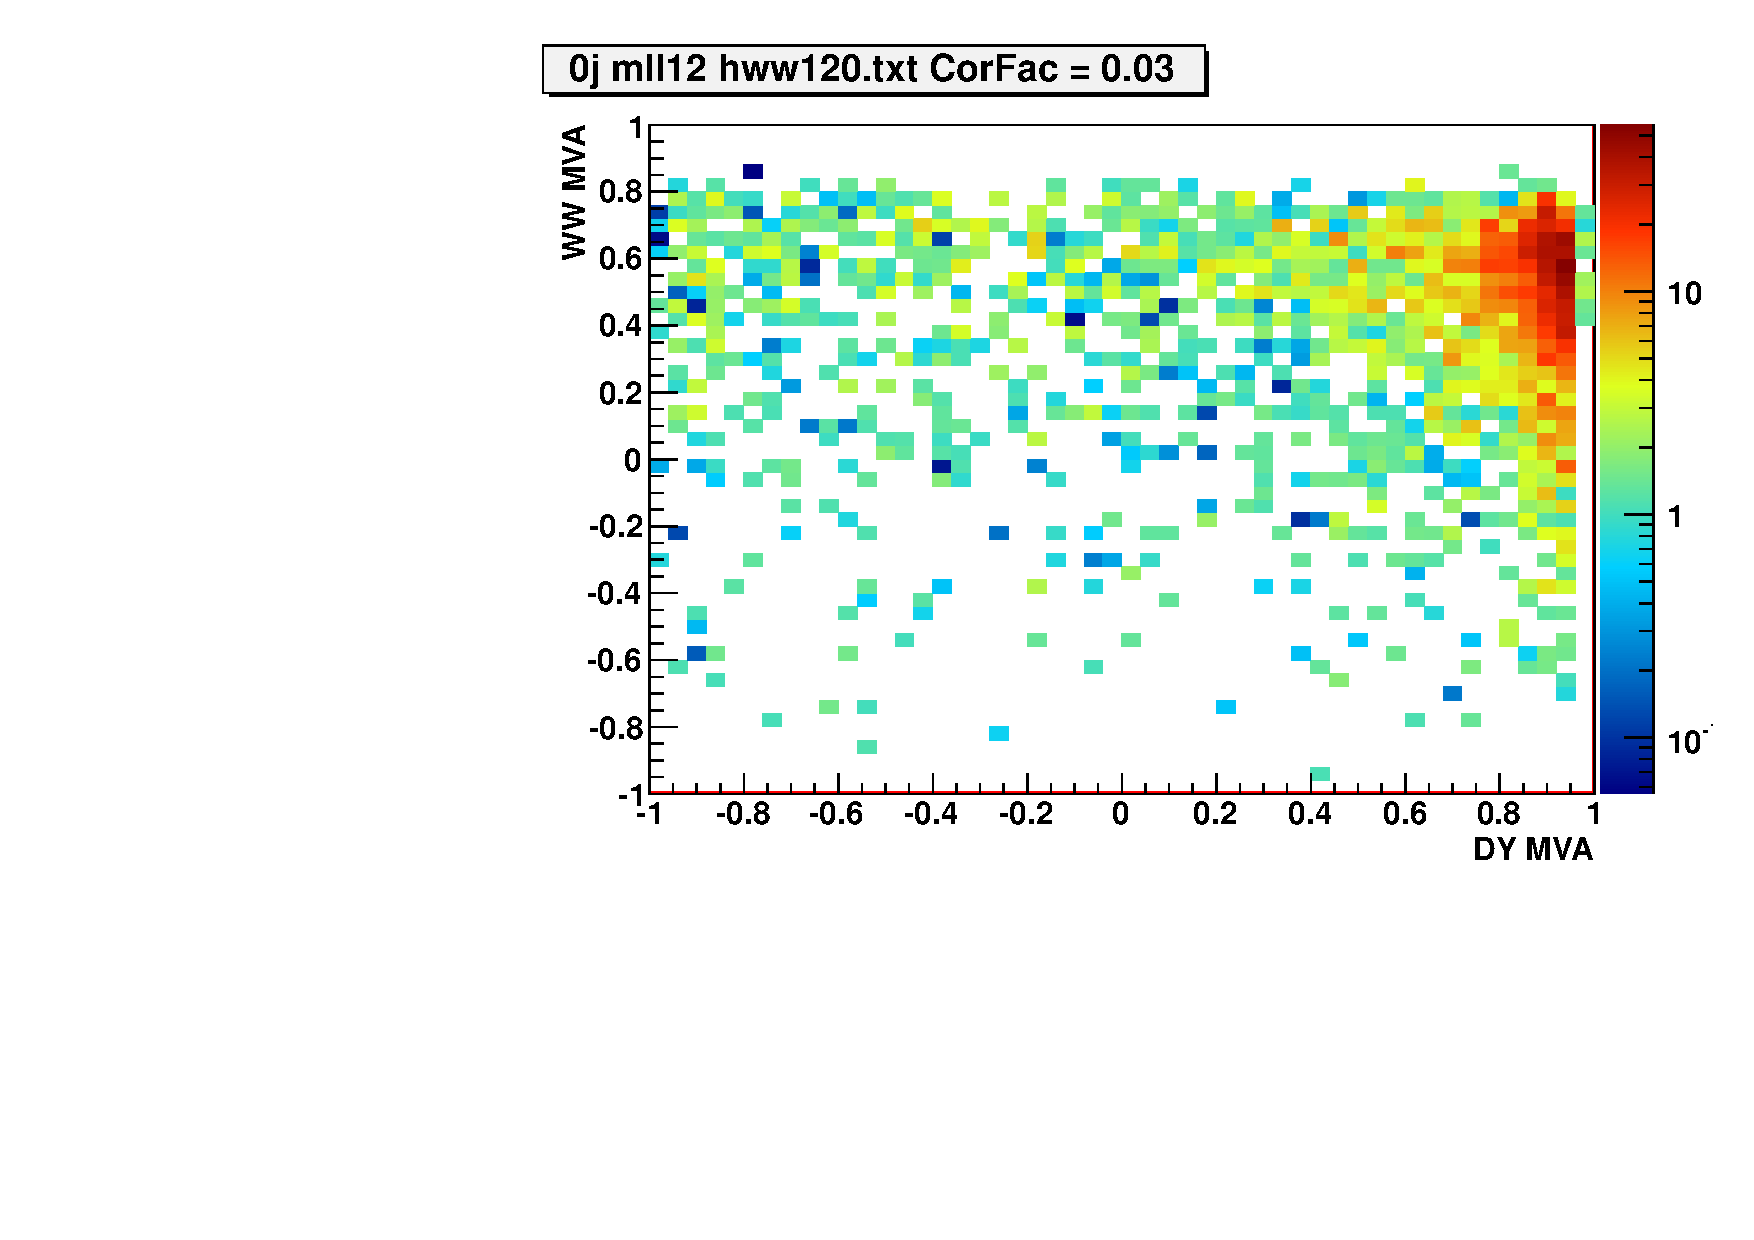
\includegraphics[width=.45\textwidth]{figures/0j_mll12_hww120.pdf}}
\subfigure[Background]{\label{subfig:0j_mll12_dy}
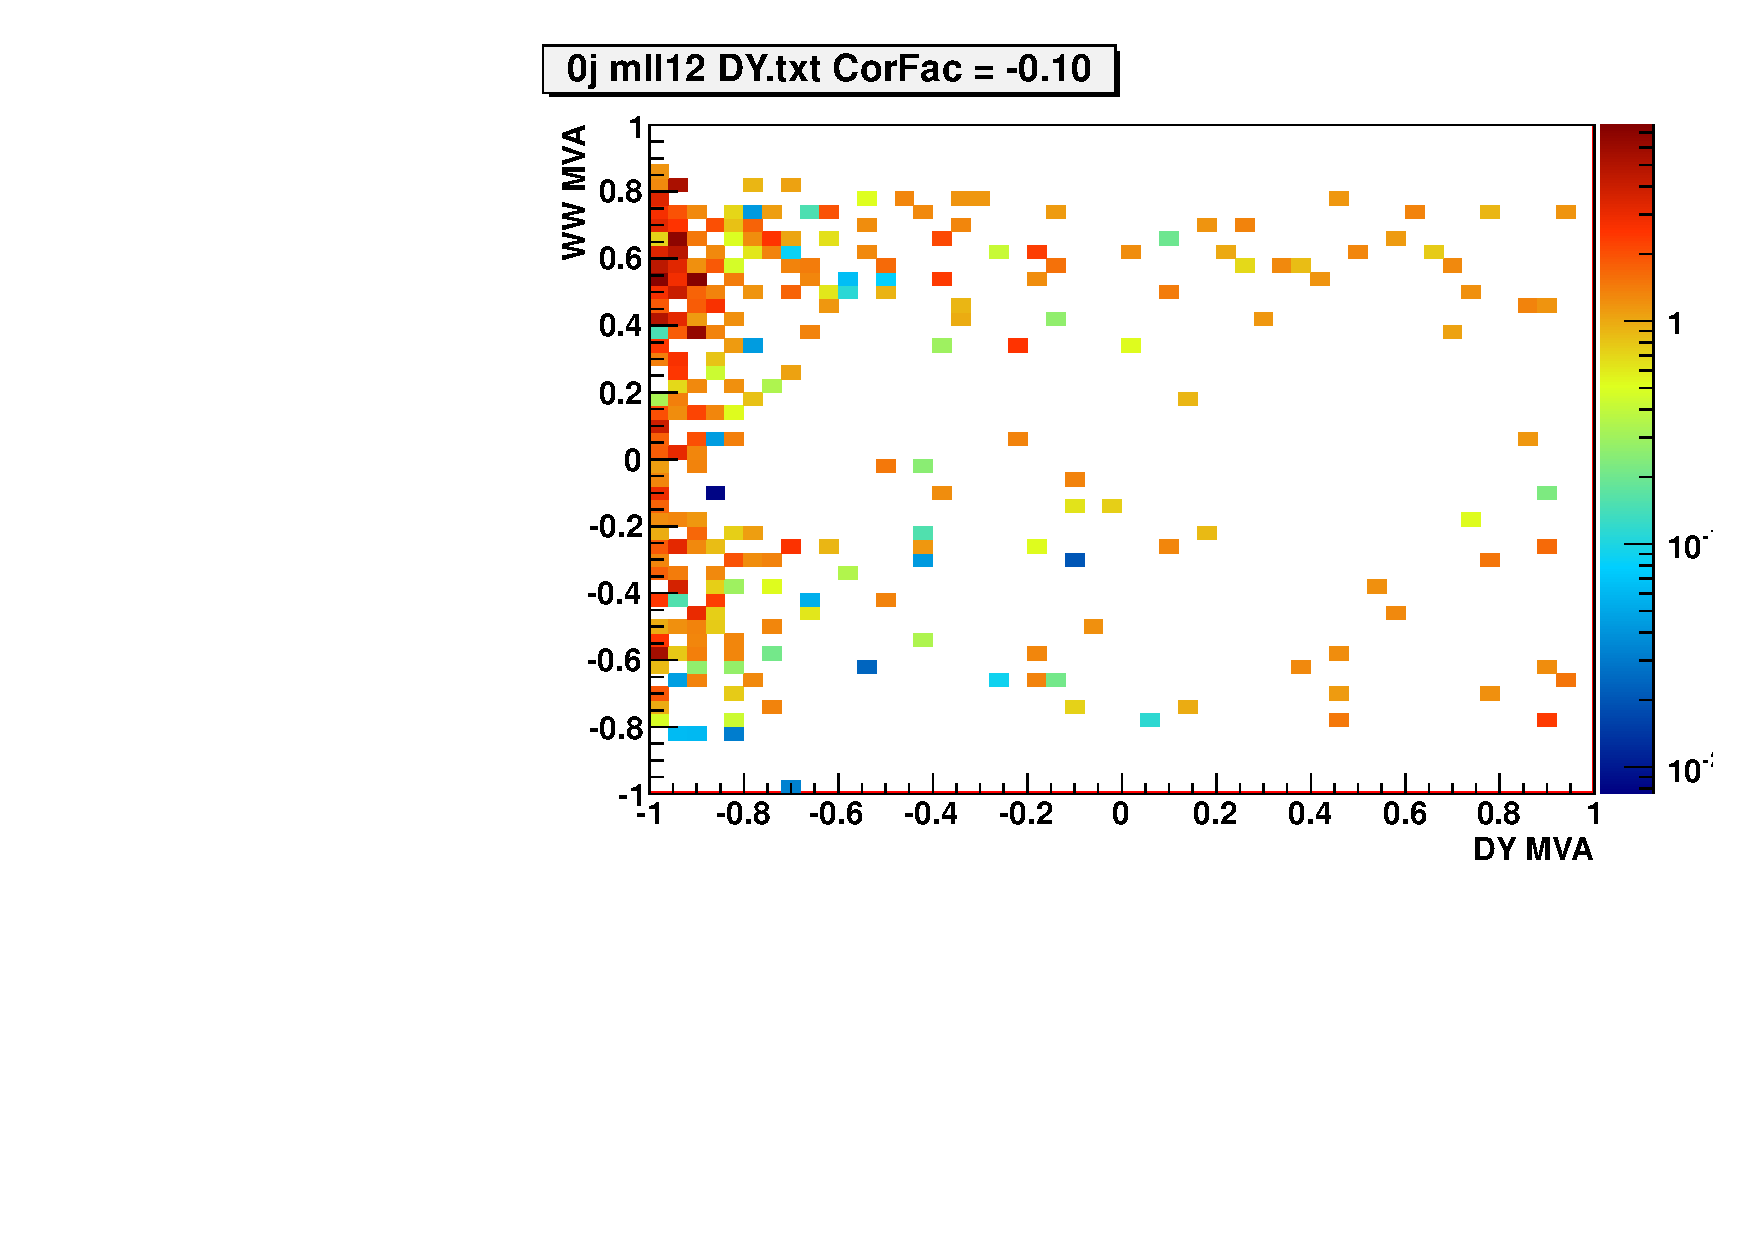
\includegraphics[width=.45\textwidth]{figures/0j_mll12_dy.pdf}}
\caption{Correlation between DY MVA and WW MVA (0-jet bin).}
\label{fig:wwmvacorr0j}
\end{center}
\end{figure}
%%%%%%%%

%%%%%%%%
\begin{figure}[!hbtp]
\begin{center}
\subfigure[Signal]{\label{subfig:1j_mll12_hww120}
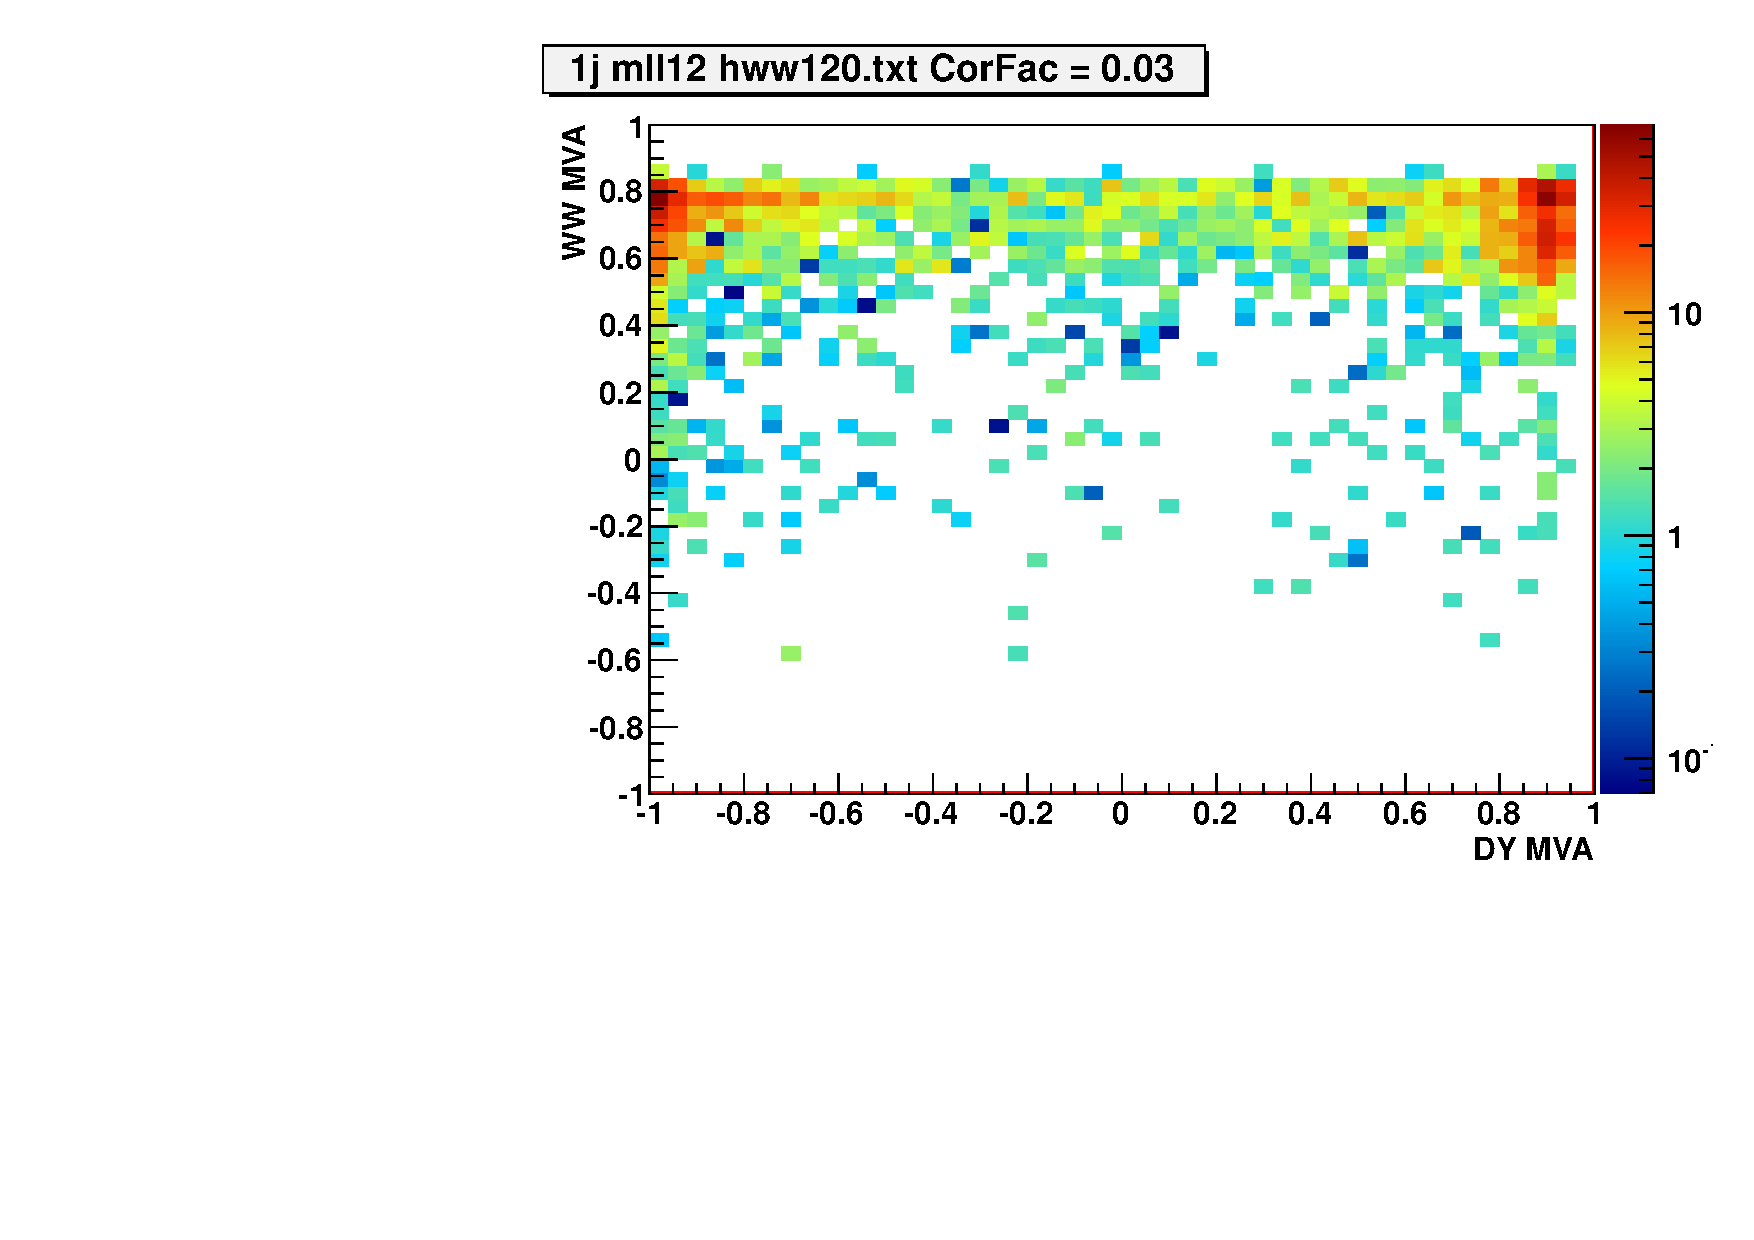
\includegraphics[width=.45\textwidth]{figures/1j_mll12_hww120.pdf}}
\subfigure[Background]{\label{subfig:1j_mll12_dy}
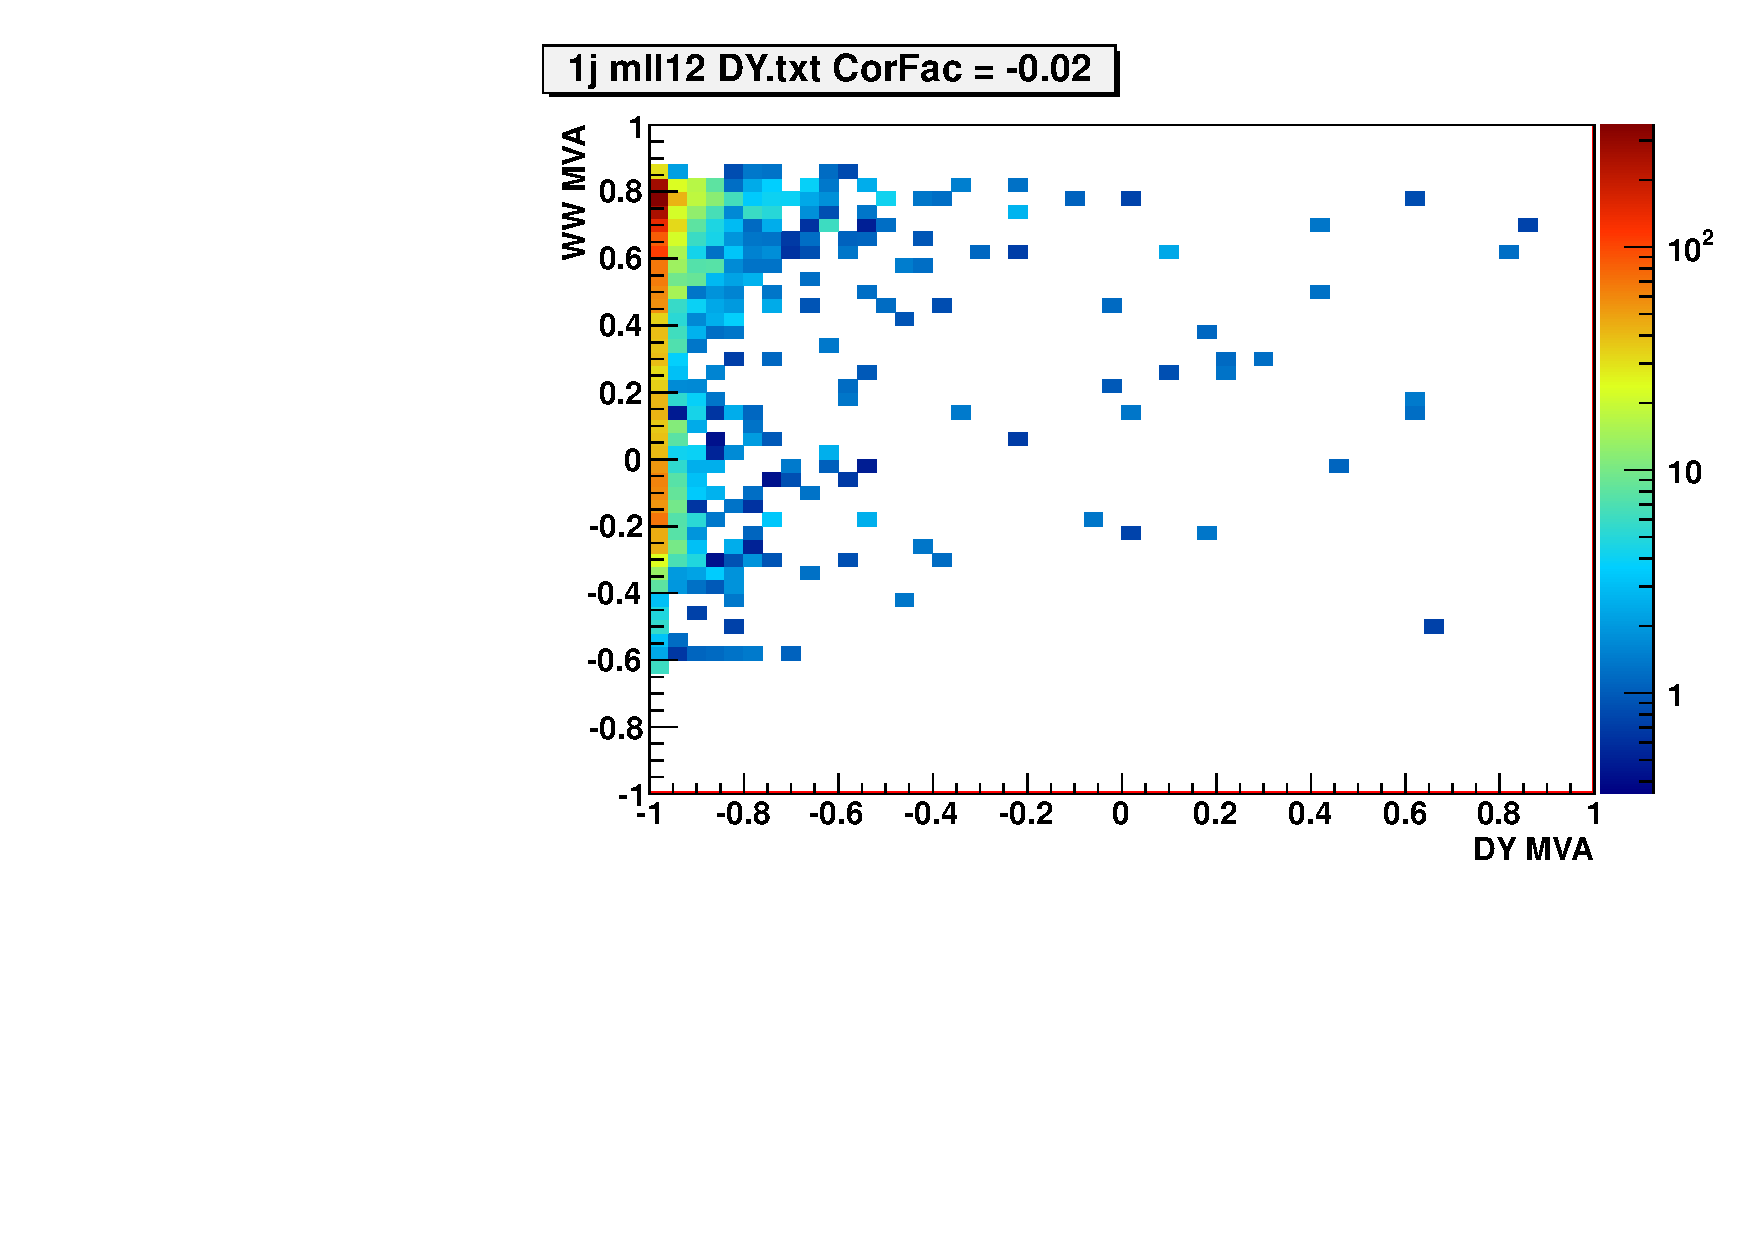
\includegraphics[width=.45\textwidth]{figures/1j_mll12_dy.pdf}}
\caption{Correlation between DY MVA and WW MVA (1-jet bin).}
\label{fig:wwmvacorr1j}
\end{center}
\end{figure}
%%%%%%%%

\clearpage
